\section{Background and Related Work}
\label{sec:related}

This section establishes the theoretical foundations for understanding feedback mechanisms in recommender systems and positions our work within the broader research landscape. We trace the evolution from early collaborative filtering approaches to contemporary deep learning and hybrid systems, highlighting key methodological developments and identifying research gaps that motivate our unified framework.

\begin{figure}[ht]
\centering
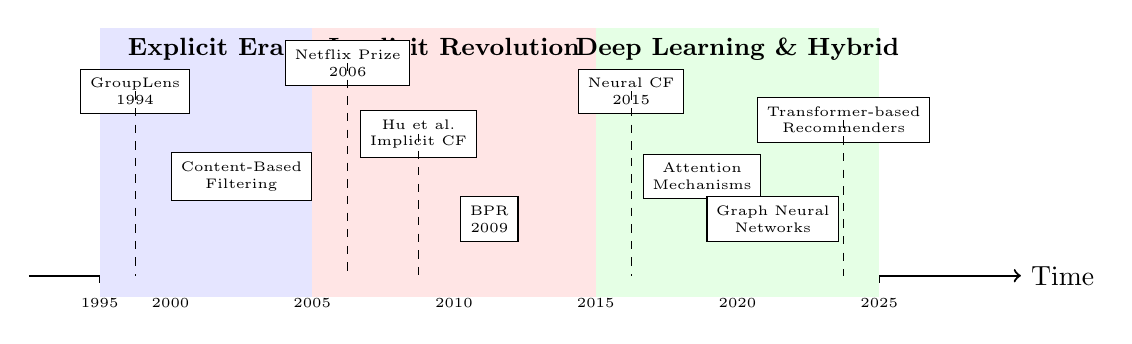
\begin{tikzpicture}[scale=0.9]
    % Timeline axis
    \draw[thick, ->] (0,0) -- (14,0) node[right] {Time};
    
    % Year markers - FIXED POSITIONING
    \draw (1,0) -- (1,-0.1) node[below, font=\tiny, yshift=-2pt] {1995};
    \draw (2,0) -- (2,-0.1) node[below, font=\tiny, yshift=-2pt] {2000};
    \draw (4,0) -- (4,-0.1) node[below, font=\tiny, yshift=-2pt] {2005};
    \draw (6,0) -- (6,-0.1) node[below, font=\tiny, yshift=-2pt] {2010};
    \draw (8,0) -- (8,-0.1) node[below, font=\tiny, yshift=-2pt] {2015};
    \draw (10,0) -- (10,-0.1) node[below, font=\tiny, yshift=-2pt] {2020};
    \draw (12,0) -- (12,-0.1) node[below, font=\tiny, yshift=-2pt] {2025};
    
    % Era backgrounds - ADJUSTED FOR BETTER POSITIONING
    \fill[blue!10] (1,-0.3) rectangle (4,3.5);
    \fill[red!10] (4,-0.3) rectangle (8,3.5);
    \fill[green!10] (8,-0.3) rectangle (12,3.5);
    
    % Era annotations
    \node[font=\small\bfseries] at (2.5,3.2) {Explicit Era};
    \node[font=\small\bfseries] at (6,3.2) {Implicit Revolution};
    \node[font=\small\bfseries] at (10,3.2) {Deep Learning \& Hybrid};
    
    % Milestones - IMPROVED VERTICAL SPACING
    \node[rectangle, draw, fill=white, align=center, font=\tiny] at (1.5,2.6) {GroupLens\\1994};
    \node[rectangle, draw, fill=white, align=center, font=\tiny] at (3,1.4) {Content-Based\\Filtering};
    \node[rectangle, draw, fill=white, align=center, font=\tiny] at (4.5,3.0) {Netflix Prize\\2006};
    \node[rectangle, draw, fill=white, align=center, font=\tiny] at (5.5,2.0) {Hu et al.\\Implicit CF};
    \node[rectangle, draw, fill=white, align=center, font=\tiny] at (6.5,0.8) {BPR\\2009};
    \node[rectangle, draw, fill=white, align=center, font=\tiny] at (8.5,2.6) {Neural CF\\2015};
    \node[rectangle, draw, fill=white, align=center, font=\tiny] at (9.5,1.4) {Attention\\Mechanisms};
    \node[rectangle, draw, fill=white, align=center, font=\tiny] at (10.5,0.8) {Graph Neural\\Networks};
    \node[rectangle, draw, fill=white, align=center, font=\tiny] at (11.5,2.2) {Transformer-based\\Recommenders};
    
    % Connecting lines
    \draw[dashed] (1.5,2.6) -- (1.5,0);
    \draw[dashed] (4.5,3.0) -- (4.5,0);
    \draw[dashed] (5.5,2.0) -- (5.5,0);
    \draw[dashed] (8.5,2.6) -- (8.5,0);
    \draw[dashed] (11.5,2.2) -- (11.5,0);
    
\end{tikzpicture}
\caption{Evolution Timeline of Recommender Systems and Feedback Mechanisms}
\Description{A timeline from 1995 to 2025 showing the evolution of recommender systems across three eras: the Explicit Era (1995-2005) featuring GroupLens and content-based filtering, the Implicit Revolution (2005-2015) with Netflix Prize and BPR, and the Deep Learning and Hybrid era (2015-2025) with neural collaborative filtering and transformer-based recommenders.}
\label{fig:evolution_timeline}
\end{figure}

Figure~\ref{fig:evolution_timeline} illustrates the historical evolution of recommender systems, highlighting three distinct eras that shaped our understanding of feedback mechanisms.

\begin{figure*}[ht]
\centering
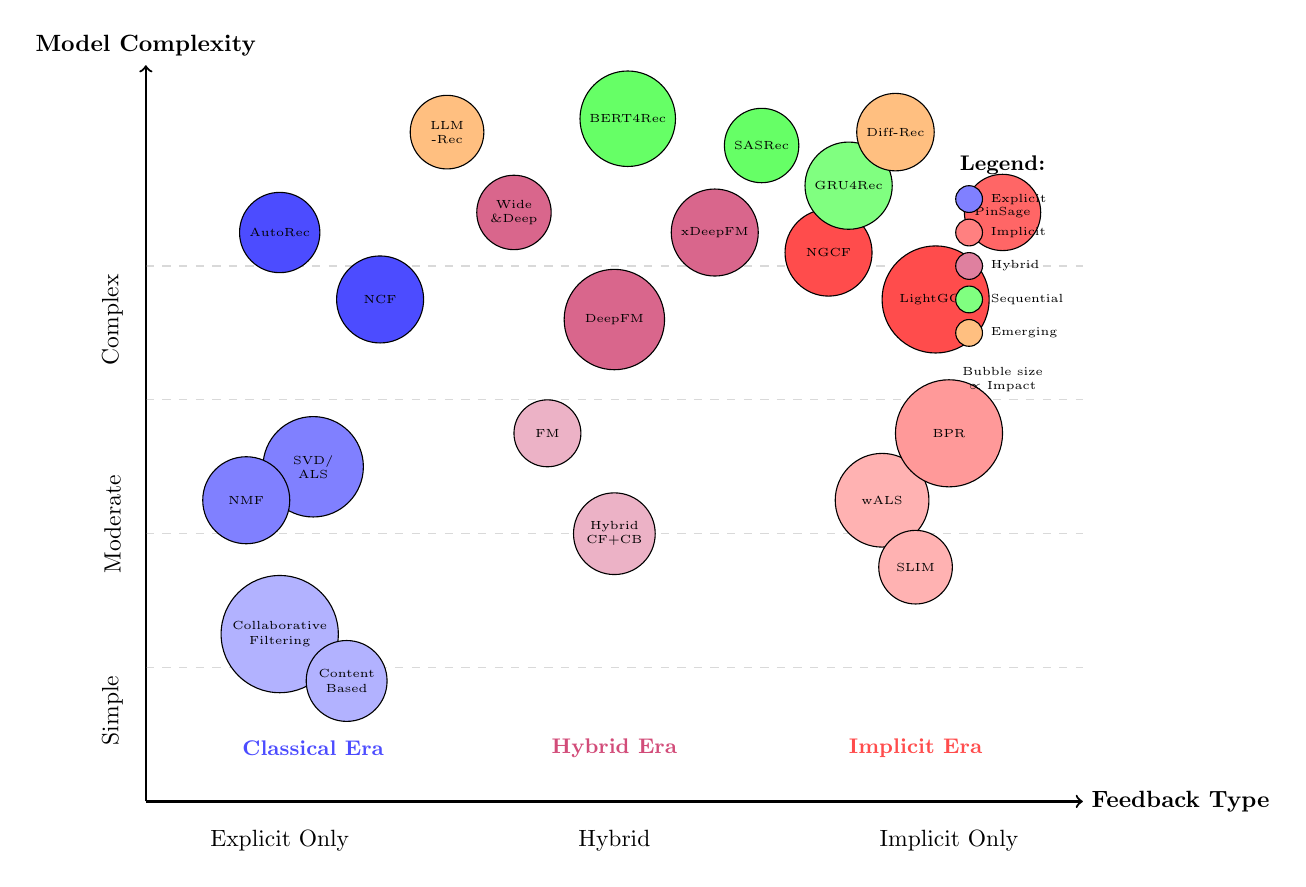
\begin{tikzpicture}[scale=0.85, transform shape]
    % Axes
    \draw[thick, ->] (0,0) -- (14,0) node[right] {\textbf{Feedback Type}};
    \draw[thick, ->] (0,0) -- (0,11) node[above] {\textbf{Model Complexity}};
    
    % Axis labels
    \node[below] at (2,-0.3) {Explicit Only};
    \node[below] at (7,-0.3) {Hybrid};
    \node[below] at (12,-0.3) {Implicit Only};
    
    \node[left, rotate=90] at (-0.5,2) {Simple};
    \node[left, rotate=90] at (-0.5,5) {Moderate};
    \node[left, rotate=90] at (-0.5,8) {Complex};
    
    % Grid
    \draw[gray, dashed, opacity=0.3] (0,2) -- (14,2);
    \draw[gray, dashed, opacity=0.3] (0,4) -- (14,4);
    \draw[gray, dashed, opacity=0.3] (0,6) -- (14,6);
    \draw[gray, dashed, opacity=0.3] (0,8) -- (14,8);
    
    % Classical Methods (Explicit, Simple)
    \node[circle, draw, fill=blue!30, minimum size=1.2cm, align=center, font=\tiny] (cf) at (2,2.5) {Collaborative\\Filtering};
    \node[circle, draw, fill=blue!30, minimum size=1cm, align=center, font=\tiny] (cbf) at (3,1.8) {Content\\Based};
    
    % Matrix Factorization (Explicit, Moderate)
    \node[circle, draw, fill=blue!50, minimum size=1.5cm, align=center, font=\tiny] (svd) at (2.5,5) {SVD/\\ALS};
    \node[circle, draw, fill=blue!50, minimum size=1.3cm, align=center, font=\tiny] (nmf) at (1.5,4.5) {NMF};
    
    % Implicit Methods (Implicit, Simple-Moderate)
    \node[circle, draw, fill=red!30, minimum size=1.4cm, align=center, font=\tiny] (wals) at (11,4.5) {wALS};
    \node[circle, draw, fill=red!40, minimum size=1.6cm, align=center, font=\tiny] (bpr) at (12,5.5) {BPR};
    \node[circle, draw, fill=red!30, minimum size=1.1cm, align=center, font=\tiny] (slim) at (11.5,3.5) {SLIM};
    
    % Hybrid Classical (Hybrid, Moderate)
    \node[circle, draw, fill=purple!30, minimum size=1.2cm, align=center, font=\tiny] (hybrid1) at (7,4) {Hybrid\\CF+CB};
    \node[circle, draw, fill=purple!30, minimum size=1cm, align=center, font=\tiny] (fm) at (6,5.5) {FM};
    
    % Deep Learning - Explicit (Complex)
    \node[circle, draw, fill=blue!70, minimum size=1.3cm, align=center, font=\tiny] (ncf) at (3.5,7.5) {NCF};
    \node[circle, draw, fill=blue!70, minimum size=1.2cm, align=center, font=\tiny] (autorec) at (2,8.5) {AutoRec};
    
    % Deep Learning - Hybrid (Complex) - ADJUSTED POSITIONS
    \node[circle, draw, fill=purple!60, minimum size=1.5cm, align=center, font=\tiny] (deepfm) at (7,7.2) {DeepFM};
    \node[circle, draw, fill=purple!60, minimum size=1.1cm, align=center, font=\tiny] (widened) at (5.5,8.8) {Wide\\\&Deep};
    \node[circle, draw, fill=purple!60, minimum size=1.1cm, align=center, font=\tiny] (xdeepfm) at (8.5,8.5) {xDeepFM};
    
    % Deep Learning - Implicit (Complex) - ADJUSTED POSITIONS
    \node[circle, draw, fill=red!70, minimum size=1.6cm, align=center, font=\tiny] (lightgcn) at (11.8,7.5) {LightGCN};
    \node[circle, draw, fill=red!70, minimum size=1.3cm, align=center, font=\tiny] (ngcf) at (10.2,8.2) {NGCF};
    \node[circle, draw, fill=red!60, minimum size=1.1cm, align=center, font=\tiny] (pinsage) at (12.8,8.8) {PinSage};
    
    % Sequential Models (Hybrid, Complex) - ADJUSTED POSITIONS
    \node[circle, draw, fill=green!60, minimum size=1.1cm, align=center, font=\tiny] (sasrec) at (9.2,9.8) {SASRec};
    \node[circle, draw, fill=green!60, minimum size=1.1cm, align=center, font=\tiny] (bert4rec) at (7.2,10.2) {BERT4Rec};
    \node[circle, draw, fill=green!50, minimum size=1cm, align=center, font=\tiny] (gru4rec) at (10.5,9.2) {GRU4Rec};
    
    % Emerging Methods (Various positions, Complex) - ADJUSTED POSITIONS
    \node[circle, draw, fill=orange!50, minimum size=1.1cm, align=center, font=\tiny] (llm) at (4.5,10) {LLM\\-Rec};
    \node[circle, draw, fill=orange!50, minimum size=1cm, align=center, font=\tiny] (diff) at (11.2,10) {Diff-Rec};
    
    % Legend - ADJUSTED POSITION FOR SCALE 0.85
    \node[font=\small\bfseries] at (12.8,9.5) {Legend:};
    \node[circle, draw, fill=blue!50, minimum size=0.4cm] at (12.3,9) {};
    \node[right, font=\tiny] at (12.5,9) {Explicit};
    \node[circle, draw, fill=red!50, minimum size=0.4cm] at (12.3,8.5) {};
    \node[right, font=\tiny] at (12.5,8.5) {Implicit};
    \node[circle, draw, fill=purple!50, minimum size=0.4cm] at (12.3,8) {};
    \node[right, font=\tiny] at (12.5,8) {Hybrid};
    \node[circle, draw, fill=green!50, minimum size=0.4cm] at (12.3,7.5) {};
    \node[right, font=\tiny] at (12.5,7.5) {Sequential};
    \node[circle, draw, fill=orange!50, minimum size=0.4cm] at (12.3,7) {};
    \node[right, font=\tiny] at (12.5,7) {Emerging};
    
    % Size indication - ADJUSTED POSITION
    \node[font=\tiny, align=center] at (12.8,6.3) {Bubble size\\$\propto$ Impact};
    
    % Era annotations
    \node[font=\small, blue!70] at (2.5,0.8) {\textbf{Classical Era}};
    \node[font=\small, purple!70] at (7,0.8) {\textbf{Hybrid Era}};
    \node[font=\small, red!70] at (11.5,0.8) {\textbf{Implicit Era}};
    
\end{tikzpicture}
\caption{Research Landscape Map: Recommendation Algorithms by Feedback Type and Complexity. Bubble size indicates research impact. Three trajectories: classical explicit methods (left), implicit approaches (right), hybrid systems (center).}
\Description{A two-dimensional scatter plot showing recommender system algorithms positioned by feedback type (explicit to implicit on x-axis) and model complexity (simple to complex on y-axis). Algorithms are shown as circles with varying sizes indicating their research impact. The plot shows clustering of classical methods in the explicit-simple region, implicit methods in the implicit-moderate region, and modern deep learning approaches in the hybrid-complex region.}
\label{fig:research_landscape}
\end{figure*}

Figure~\ref{fig:research_landscape} provides a comprehensive visualization of the recommender systems research landscape, positioning major algorithmic approaches according to their feedback type specialization and model complexity. This two-dimensional representation reveals clear evolutionary patterns and research clusters.

\subsection{Foundations of Recommender Systems}

Recommender systems emerged in the 1990s as a response to information overload in digital environments. Early systems focused primarily on explicit feedback due to its clear semantic interpretation and the limited computational resources available for processing large-scale behavioral data~\cite{resnick1994grouplens,shardanand1995social}.

\subsubsection{Collaborative Filtering Paradigms}
The foundational work of Resnick et al.~\cite{resnick1994grouplens} established collaborative filtering as the dominant paradigm for recommendation systems. Their GroupLens system demonstrated that user preferences could be inferred from rating patterns, leading to two primary approaches:

\textbf{Memory-based methods} compute recommendations directly from user-item rating matrices using similarity measures. Neighborhood-based collaborative filtering identifies similar users (user-based CF) or items (item-based CF) to make predictions~\cite{herlocker1999algorithmic,sarwar2001item}.

\textbf{Model-based methods} learn latent representations from rating data. Matrix factorization techniques, particularly after the Netflix Prize~\cite{bennett2007netflix}, became the dominant approach for explicit feedback systems, with methods like SVD and Non-negative Matrix Factorization (NMF) achieving state-of-the-art performance~\cite{koren2009matrix,lee1999learning}.

\subsubsection{Content-Based and Hybrid Approaches}
Parallel to collaborative filtering, content-based systems emerged that recommend items similar to those previously preferred by users~\cite{pazzani2007content}. Hybrid systems combining collaborative and content-based approaches addressed limitations of individual methods, particularly the cold-start problem~\cite{burke2002hybrid,adomavicius2005toward}.

\subsection{The Implicit Feedback Revolution}

The transition to web-scale applications in the 2000s revealed fundamental limitations of explicit feedback approaches, leading to increased focus on implicit signals.

\subsubsection{Foundational Implicit Feedback Work}
Hu et al.~\cite{hu2008collaborative} provided the first systematic treatment of implicit feedback in recommender systems. Their weighted matrix factorization approach addressed key challenges:
\begin{itemize}
    \item \textbf{No negative feedback}: Unlike explicit ratings, implicit feedback only provides positive signals
    \item \textbf{Varying confidence}: Different actions indicate varying levels of preference strength
    \item \textbf{Numerical value interpretation}: Raw counts (views, clicks) require careful transformation
\end{itemize}

Pan et al.~\cite{pan2008one} formalized implicit feedback as a one-class learning problem, developing techniques specifically designed for scenarios where only positive examples are observed. This work established the theoretical foundation for subsequent implicit feedback research.

\subsubsection{Ranking-Based Approaches}
The recognition that implicit feedback is better suited for ranking than rating prediction led to significant methodological developments. Rendle et al.~\cite{rendle2009bpr} introduced Bayesian Personalized Ranking (BPR), which optimizes for item ranking rather than rating prediction. BPR's pairwise learning approach became widely adopted for implicit feedback systems.

\subsection{Algorithmic Evolution and Deep Learning}

The 2010s witnessed rapid evolution in recommendation algorithms, driven by advances in machine learning and computational capabilities.

\subsubsection{Matrix Factorization Extensions}
Building on basic matrix factorization, researchers developed sophisticated extensions:
\begin{itemize}
    \item \textbf{Temporal dynamics}: Koren~\cite{koren2009collaborative} incorporated time-varying preferences
    \item \textbf{Regularization techniques}: Various approaches addressed overfitting and improved generalization
    \item \textbf{Factorization machines}: Rendle~\cite{rendle2012factorization} generalized matrix factorization to arbitrary feature interactions
\end{itemize}

\subsubsection{Deep Learning Transformation}
The application of deep learning to recommender systems began in earnest around 2015, revolutionizing both explicit and implicit feedback processing:

\textbf{Neural Collaborative Filtering}: He et al.~\cite{he2017neural} demonstrated that neural networks could effectively model user-item interactions, leading to improved performance over traditional matrix factorization.

\textbf{Autoencoders}: AutoRec~\cite{sedhain2015autorec} and subsequent autoencoder-based approaches showed promise for both explicit and implicit feedback scenarios.

\textbf{Recurrent Neural Networks}: Session-based recommendation systems leveraged RNNs to model sequential user behavior~\cite{hidasi2015session}, particularly relevant for implicit feedback scenarios.

\textbf{Attention Mechanisms}: The introduction of attention mechanisms enabled more sophisticated modeling of user preferences and item characteristics~\cite{chen2017attentive}.

\subsubsection{Graph-Based Approaches}
Recent years have seen significant interest in graph-based recommendation methods:
\begin{itemize}
    \item \textbf{Graph Neural Networks}: Methods like LightGCN~\cite{he2020lightgcn} leverage graph structure in user-item interactions
    \item \textbf{Knowledge Graphs}: Integration of external knowledge to enhance recommendation quality~\cite{wang2019kgat}
    \item \textbf{Social Networks}: Incorporation of social signals into recommendation algorithms~\cite{ma2011learning}
\end{itemize}

\subsection{Hybrid and Multi-Modal Systems}

The limitations of single feedback type systems led to increased interest in hybrid approaches that combine multiple signal sources.

\subsubsection{Early Hybrid Systems}
Burke~\cite{burke2002hybrid} established the theoretical framework for hybrid recommender systems, identifying several combination strategies:
\begin{itemize}
    \item \textbf{Weighted}: Linear combination of multiple recommendation sources
    \item \textbf{Switching}: Dynamic selection based on situation
    \item \textbf{Mixed}: Parallel presentation of recommendations from different sources
    \item \textbf{Feature combination}: Integration at the feature level
    \item \textbf{Cascade}: Sequential refinement of recommendations
    \item \textbf{Feature augmentation}: One technique adds features for another
    \item \textbf{Meta-level}: One technique serves as input to another
\end{itemize}

\subsubsection{Modern Hybrid Approaches}
Contemporary hybrid systems leverage deep learning to seamlessly integrate multiple feedback types:
\begin{itemize}
    \item \textbf{Multi-task learning}: Simultaneous optimization for different feedback types~\cite{ma2018modeling}
    \item \textbf{Attention-based fusion}: Learning optimal combination weights~\cite{chen2017attentive}
    \item \textbf{Cross-domain transfer}: Leveraging feedback from related domains~\cite{zhu2019transfer}
\end{itemize}

\subsubsection{Multi-Modal Integration}
Recent work extends beyond traditional feedback to incorporate diverse signal types:
\begin{itemize}
    \item \textbf{Textual reviews}: Natural language processing for review sentiment and topics~\cite{zheng2018joint}
    \item \textbf{Visual content}: Computer vision for image and video recommendations~\cite{wei2021contrastive}
    \item \textbf{Audio features}: Music recommendation using audio signal processing~\cite{van2013deep}
    \item \textbf{Contextual information}: Location, time, and device context~\cite{adomavicius2011context}
\end{itemize}

\subsection{Evaluation and Bias Considerations}

As recommender systems matured, the research community recognized critical issues in evaluation methodologies and fairness considerations.

\subsubsection{Evaluation Challenges}
Herlocker et al.~\cite{herlocker2004evaluating} provided the first comprehensive framework for evaluating collaborative filtering systems, highlighting challenges that persist today:
\begin{itemize}
    \item \textbf{Offline vs. online evaluation}: Differences between historical data analysis and live user studies
    \item \textbf{Metric selection}: Choosing appropriate metrics for different system goals
    \item \textbf{Statistical significance}: Ensuring reliable performance comparisons
\end{itemize}

Recent work by Dacrema et al.~\cite{dacrema2019we} raised concerns about reproducibility and fair comparison in deep learning-based recommendation research, highlighting the need for more rigorous evaluation practices.

\subsubsection{Bias and Fairness}
The recognition of bias in recommender systems has led to significant research attention:
\begin{itemize}
    \item \textbf{Selection bias}: Users choose which items to rate, creating biased training data~\cite{marlin2007collaborative}
    \item \textbf{Popularity bias}: Over-representation of popular items in recommendations~\cite{abdollahpouri2019unfairness}
    \item \textbf{Demographic bias}: Differential performance across user groups~\cite{ekstrand2022fairness}
    \item \textbf{Exposure bias}: Limited item exposure affects feedback collection~\cite{joachims2017accurately}
\end{itemize}

\subsection{Emerging Trends and Future Directions}

Recent research has identified several emerging trends that will shape the future of recommender systems:

\subsubsection{Privacy-Preserving Recommendations}
Growing privacy concerns have led to development of privacy-preserving recommendation techniques:
\begin{itemize}
    \item \textbf{Federated learning}: Distributed training without centralizing user data~\cite{chai2020secure}
    \item \textbf{Differential privacy}: Mathematical privacy guarantees for recommendation algorithms~\cite{mcsherry2009differentially}
    \item \textbf{Homomorphic encryption}: Computing on encrypted recommendation data~\cite{erkin2012privacy}
\end{itemize}

\subsubsection{Causal Inference and Debias}
Application of causal inference methods to address bias in recommendation systems:
\begin{itemize}
    \item \textbf{Causal embeddings}: Learning representations that capture causal relationships~\cite{bonner2018causal}
    \item \textbf{Counterfactual reasoning}: Estimating what would have happened under different conditions~\cite{schnabel2016recommendations}
    \item \textbf{Debiasing techniques}: Methods to reduce various forms of bias in recommendations~\cite{chen2020bias}
\end{itemize}

\subsubsection{Large Language Models and Foundation Models}
The emergence of large language models presents new opportunities for recommendation systems:
\begin{itemize}
    \item \textbf{Natural language interfaces}: Conversational recommendation systems~\cite{gao2021advances}
    \item \textbf{Zero-shot recommendations}: Leveraging pre-trained models for new domains~\cite{hou2023large}
    \item \textbf{Explanation generation}: Automatic generation of recommendation explanations~\cite{zhang2020explainable}
\end{itemize}

\subsection{Research Gaps and Motivations}

Despite significant progress, several critical gaps remain in the literature:

\subsubsection{Lack of Unified Framework}
Most research treats implicit and explicit feedback as separate problems, with limited systematic comparison of their fundamental properties and optimal application contexts. This fragmentation hinders principled system design and fair algorithmic comparison.

\subsubsection{Inadequate Evaluation for Hybrid Systems}
Current evaluation methodologies are poorly suited for hybrid systems that combine multiple feedback types. Standard metrics may not capture the nuanced trade-offs and complementary strengths of different feedback sources.

\subsubsection{Limited Real-World Analysis}
Most research focuses on algorithmic development with limited analysis of real-world deployment patterns and their relationship to feedback characteristics. This gap limits the practical applicability of research findings.

\subsubsection{Insufficient Bias Analysis}
While bias in individual feedback types has received attention, the differential bias characteristics of implicit versus explicit feedback and their implications for hybrid systems remain underexplored.

These gaps motivate our comprehensive survey and unified framework, which aims to establish theoretical foundations for systematic comparison and optimal utilization of different feedback types in modern recommender systems.

\paragraph{Privacy and Federated Learning}
Privacy concerns have driven federated learning approaches~\cite{chai2020secure} and differential privacy techniques~\cite{jia2021privacy}, enabling feedback processing without centralized data collection.

\subsection{Key Research Themes and Methodological Developments}

\subsubsection{Feedback Modeling Paradigms}

Research on feedback modeling has evolved through several distinct phases, each building upon previous advances while addressing new challenges.

\paragraph{Classical Collaborative Filtering}
Early work established collaborative filtering as the foundation of recommender systems. User-based and item-based methods~\cite{sarwar2001item, breese1998empirical} identified similar users or items to make predictions. Matrix factorization techniques~\cite{koren2009matrix} provided scalable solutions for sparse data, with extensions for temporal dynamics~\cite{koren2010collaborative}.

\paragraph{Neural and Deep Learning Approaches}
Deep learning transformed feedback modeling by enabling complex, non-linear interactions. Neural Collaborative Filtering~\cite{he2017neural} combined matrix factorization with neural networks, while Wide \& Deep~\cite{cheng2016wide} integrated memorization and generalization. Autoencoder-based methods~\cite{sedhain2015autorec} proved effective for implicit feedback reconstruction.

\paragraph{Sequential and Temporal Modeling}
Sequential patterns in user behavior led to specialized modeling approaches. Recurrent Neural Networks~\cite{hidasi2015session} and Transformers~\cite{kang2018self, sun2019bert4rec} capture temporal dependencies, while attention mechanisms~\cite{kang2018self} identify relevant historical interactions.

\paragraph{Graph-Based and Relational Methods}
Graph Neural Networks model recommender systems as heterogeneous graphs. Methods like NGCF~\cite{wang2019neural} and LightGCN~\cite{he2020lightgcn} propagate information through user-item interaction graphs, while HyperGCN~\cite{hypergcn} handles hypergraph structures.

\paragraph{Self-Supervised and Contrastive Learning}
Recent advances leverage self-supervised learning for representation learning. Contrastive objectives~\cite{yao2021self, xie2022contrastive} learn from implicit feedback patterns, while masked prediction tasks~\cite{hou2022towards} reconstruct missing interactions.

\subsubsection{Hybrid Feedback Integration Strategies}

Combining multiple feedback types presents unique challenges and opportunities, with research focusing on principled integration approaches.

\paragraph{Multi-Task Learning Frameworks}
Joint optimization of implicit and explicit objectives has proven effective. Methods like those in~\cite{ma2011learning, zhao2015improving} share representations across feedback types, while attention-based approaches~\cite{chen2017attentive, liu2018stamp} dynamically weight different signals.

\paragraph{Knowledge Distillation and Transfer}
Knowledge distillation transfers insights between feedback modalities~\cite{zhang2020knowledge}. Teacher-student frameworks enable implicit feedback models to benefit from explicit feedback supervision, even when explicit data is limited.

\paragraph{Multimodal Fusion Techniques}
Modern systems integrate diverse feedback sources. Textual reviews enhance behavioral signals~\cite{liu2022multimodal}, while visual features provide complementary information~\cite{wei2021contrastive}. Cross-modal alignment techniques learn unified representations across modalities.

\subsubsection{Evaluation Methodologies and Bias Analysis}

Evaluation frameworks have evolved from simple accuracy metrics to comprehensive assessments of system performance and societal impact.

\paragraph{Metrics Development and Standardization}
Beyond traditional metrics like RMSE and precision@K, research has developed comprehensive evaluation suites. Novelty and diversity metrics~\cite{castells2011novelty} assess recommendation quality beyond accuracy, while fairness metrics~\cite{ge2020understanding} evaluate equitable treatment.

\paragraph{Bias Detection and Mitigation}
Systematic analysis of biases has become crucial. Popularity bias~\cite{abdollahpouri2019unfairness}, position bias~\cite{wang2021user}, and selection bias~\cite{schnabel2016recommendations} affect recommendation quality. Debiasing techniques include reweighting~\cite{wang2021user} and adversarial approaches~\cite{zehlike2020reducing}.

\paragraph{User-Centric Evaluation}
User studies and behavioral analysis complement algorithmic evaluation. Work on user satisfaction~\cite{knijnenburg2012explaining}, trust~\cite{pu2011user}, and behavioral responses provides insights into real-world effectiveness.

\subsubsection{Domain-Specific Applications and Case Studies}

Feedback mechanisms vary significantly across application domains, requiring specialized approaches and evaluation criteria.

\paragraph{E-commerce and Retail}
Purchase prediction dominates e-commerce recommendations. Amazon's system leverages purchase histories and browsing patterns~\cite{linden2003amazon}, while modern approaches incorporate multimodal signals~\cite{covington2016deep}. Basket recommendation and cross-selling present unique challenges.

\paragraph{Entertainment and Streaming}
Content discovery in video and music streaming relies heavily on implicit feedback. Netflix's system combines viewing behaviors with explicit ratings~\cite{gomez2015netflix}, while Spotify's algorithmic playlists leverage listening patterns~\cite{van2013deep}. Completion prediction and abandonment analysis are critical.

\paragraph{Social Media and News}
Feed optimization balances engagement with quality. Facebook and Twitter systems process massive implicit signals from user interactions, while news recommenders must balance timeliness, diversity, and credibility. 

News recommendation has emerged as a critical research area with unique challenges stemming from content velocity, diversity requirements, and societal impact. The development of large-scale datasets like MIND~\cite{wu2020mind_news} (Microsoft News Dataset with 160K+ articles and 15M+ interactions) and Adressa~\cite{gulla2017adressa} (Norwegian news portal data with detailed engagement metrics) has accelerated research by providing standardized benchmarks for reproducible evaluation.

Neural approaches have proven particularly effective for news recommendation. NPA~\cite{wu2019npa} introduced personalized attention mechanisms that adapt to individual user preferences, while multi-view learning methods~\cite{wu2019neural} effectively integrate textual content, categorical information, and entity knowledge. Recent work leverages pre-trained language models~\cite{wu2021empowering} for enhanced semantic understanding and applies graph neural networks~\cite{hu2020graph} to model complex user-article interaction patterns.

News recommendation relies almost exclusively on implicit feedback (clicks, dwell time, scrolling) due to the low engagement threshold for explicit rating collection. This creates unique challenges: clickbait detection, position bias mitigation, and distinguishing genuine interest from curiosity clicks. Causal inference methods~\cite{qi2021causal} have emerged to address these biases, employing inverse propensity scoring and counterfactual reasoning to improve recommendation quality.

Echo chamber mitigation remains a significant challenge, as over-personalization risks creating filter bubbles that limit exposure to diverse viewpoints. Balancing engagement optimization with diversity, serendipity, and editorial priorities requires multi-objective frameworks that go beyond simple click-through rate maximization.

\paragraph{Education and Learning}
Personalized learning paths require careful feedback integration. Systems adapt content difficulty based on performance~\cite{tang2019towards}, while peer assessment and progress tracking provide additional signals.

\subsection{Research Gaps, Open Challenges, and Emerging Directions}

Despite extensive research, significant gaps remain that present opportunities for future work.

\subsubsection{Theoretical Foundations and Fundamental Limits}

\begin{itemize}
    \item \textbf{Feedback Quality Bounds}: Limited understanding of fundamental limits on recommendation accuracy given different feedback types
    \item \textbf{Unified Theoretical Frameworks}: Lack of comprehensive theories explaining feedback type interactions and trade-offs
    \item \textbf{Causal Inference}: Insufficient understanding of causal relationships between feedback and user satisfaction
    \item \textbf{Information-Theoretic Limits}: Bounds on recommendation performance given feedback constraints
\end{itemize}

\subsubsection{Practical Challenges and Scalability Issues}

\begin{itemize}
    \item \textbf{Cross-Domain Transfer}: Effective transfer of feedback knowledge across different application domains
    \item \textbf{Longitudinal Dynamics}: Adaptation to evolving user preferences and feedback patterns over extended periods
    \item \textbf{Privacy-Utility Trade-offs}: Balancing rich feedback collection with user privacy requirements
    \item \textbf{Fairness at Scale}: Ensuring equitable treatment across diverse user populations in large-scale systems
    \item \textbf{Real-Time Processing}: Sub-second response times for streaming feedback and dynamic adaptation
\end{itemize}

\subsubsection{Emerging Research Directions}

\begin{itemize}
    \item \textbf{Large Language Model Integration}: Leveraging LLMs for feedback interpretation, natural language interfaces, and conversational recommendations
    \item \textbf{Multimodal and Cross-Modal Learning}: Integrating diverse feedback modalities including physiological signals and brain-computer interfaces
    \item \textbf{Self-Supervised Learning}: Developing unsupervised approaches that maximize information extraction from implicit feedback
    \item \textbf{Federated and Privacy-Preserving Methods}: Enabling feedback processing without centralized data collection
    \item \textbf{Causal Recommendation}: Moving beyond correlation to causal understanding of user preferences
    \item \textbf{Sustainable AI}: Energy-efficient recommendation systems that minimize computational and environmental costs
\end{itemize}

\subsection{Survey Contributions and Positioning}

This survey advances the field by providing a comprehensive synthesis that bridges historical foundations with contemporary advances. To contextualize our contributions, Table~\ref{tab:survey_comparison} compares this work with related survey papers in the recommender systems literature.

\begin{table*}[ht]
\centering
\tiny
\caption{Comparison with Related Survey Papers}
\label{tab:survey_comparison}
\begin{tabular}{@{}lcccccccc@{}}
\toprule
Survey & Year & Papers & Implicit & Explicit & Hybrid & Eval & Bias & Domains \\
 & & Covered & Focus & Focus & Focus & Metrics & Analysis & Covered \\
\midrule
\multicolumn{9}{l}{\textit{\textbf{General Recommender Systems Surveys}}} \\
\midrule
Adomavicius \& Tuzhilin & 2005 & 80+ & Low & High & No & Basic & No & 3 \\
Ricci et al. (Handbook) & 2015 & 150+ & Med & High & Low & Med & Low & 5 \\
Zhang et al. & 2019 & 100+ & Med & Med & Med & Med & Low & 4 \\
\midrule
\multicolumn{9}{l}{\textit{\textbf{Specialized Feedback Surveys}}} \\
\midrule
Pan et al. & 2016 & 40 & High & No & No & High & Med & 2 \\
Implicit Feedback Focus & & & & & & & & \\
\midrule
\multicolumn{9}{l}{\textit{\textbf{Deep Learning for RecSys}}} \\
\midrule
Zhang et al. & 2019 & 100+ & Med & Low & Low & Low & No & 4 \\
Batmaz et al. & 2019 & 80+ & Med & Med & Low & Low & No & 3 \\
Wu et al. & 2022 & 120+ & High & Low & Med & Med & Low & 5 \\
\midrule
\multicolumn{9}{l}{\textit{\textbf{Evaluation and Bias}}} \\
\midrule
Herlocker et al. & 2004 & 50 & Low & High & No & High & No & 2 \\
Gunawardana \& Shani & 2015 & 60 & Med & Med & No & High & Med & 3 \\
Chen et al. & 2023 & 70 & Med & Med & Low & High & High & 4 \\
\midrule
\multicolumn{9}{l}{\textit{\textbf{Domain-Specific Surveys}}} \\
\midrule
Gomez-Uribe \& Hunt & 2016 & 30 & High & Med & Med & Med & No & 1 \\
(Netflix) & & & & & & & & \\
Schedl et al. & 2018 & 90+ & High & Low & Low & Med & No & 1 \\
(Music) & & & & & & & & \\
\midrule
\multicolumn{9}{l}{\textbf{\textit{This Survey (2025)}}} \\
\midrule
Our Work & 2025 & \textbf{147} & \textbf{High} & \textbf{High} & \textbf{High} & \textbf{High} & \textbf{High} & \textbf{6} \\
\bottomrule
\multicolumn{9}{l}{\scriptsize \textit{Legend: High = Comprehensive coverage; Med = Moderate coverage; Low = Limited coverage; No = Not covered}} \\
\multicolumn{9}{l}{\scriptsize \textit{Eval Metrics = Evaluation methodology coverage; Bias Analysis = Bias detection/mitigation coverage}} \\
\end{tabular}
\end{table*}

\textbf{Key Differentiators of This Survey:}

\begin{enumerate}
    \item \textbf{Unified Feedback-Centric Perspective}: Unlike prior surveys that treat feedback types separately or emphasize algorithmic approaches, we establish feedback mechanisms as the primary organizing principle, enabling systematic comparison and principled design choices.
    
    \item \textbf{Comprehensive Hybrid Coverage}: First survey to provide extensive analysis of hybrid approaches (combining implicit and explicit feedback) with specific fusion strategies, integration patterns, and comparative performance analysis.
    
    \item \textbf{Bias-Aware Evaluation Framework}: Extensive treatment of bias detection and mitigation tailored to different feedback types—addressing selection, popularity, and position bias with feedback-specific protocols.
    
    \item \textbf{Modern Architecture Coverage}: Includes latest developments (2020-2025) such as transformer-based recommenders, LLM integration, federated learning, and diffusion models—absent from earlier surveys.
    
    \item \textbf{Practitioner-Oriented Guidance}: Decision frameworks, implementation checklists, and domain-specific best practices designed for system architects and practitioners, not just researchers.
    
    \item \textbf{Multi-Domain Analysis}: Systematic coverage across six major application domains (e-commerce, streaming, social media, news, education, healthcare) with domain-specific feedback characteristics and optimal strategies.
    
    \item \textbf{Reproducibility Resources}: Comprehensive dataset characterization, preprocessing guidelines, and benchmark comparisons to facilitate reproducible research.
    
    \item \textbf{Forward-Looking Research Agenda}: Identification of emerging challenges in privacy-preserving recommendations, fairness-aware systems, multimodal integration, and explainable AI.
\end{enumerate}

\textbf{Survey Contributions Summary:}

\begin{itemize}
    \item \textbf{Comprehensive Coverage}: Integration of 147 publications from 2010-2025 with historical context
    \item \textbf{Unified Framework}: Five-dimensional taxonomy bridging implicit and explicit feedback characteristics
    \item \textbf{Methodological Synthesis}: Comprehensive review of algorithmic approaches from classical to cutting-edge methods
    \item \textbf{Practical Insights}: Implementation guidance and best practices for real-world deployment
    \item \textbf{Future Roadmap}: Identification of research directions and emerging opportunities
    \item \textbf{Cross-Disciplinary Perspective}: Integration of insights from computer science, psychology, and behavioral economics
\end{itemize}

Our analysis draws from major conferences (ACM RecSys, SIGIR, KDD, WWW, NeurIPS) and journals (ACM TORS, IEEE TKDE, JMLR, Nature Machine Intelligence), with emphasis on rigorous, peer-reviewed work while maintaining accessibility for diverse audiences.